\documentclass[aspectratio=169]{beamer}
\usepackage{simplebeamer}

\begin{document}

\begin{frame}

    \begin{center}
        \titletext{Coalescent inference of HIV transmission history}

        \vfill

        Raymond Heil

        T-6: Theoretical Biology and Biophysics

        Emma Goldberg, Thomas Leitner

        \vfill

        \scriptsize{20 July 2022}

    \end{center}

    %\ftnA{LA-UR-XX-XXXXX} % add this back in when I get an LA-UR

\end{frame}

%--------------------------------------------------
\section{Why this project?}
%--------------------------------------------------

\begin{frame} \frametitle{\insertsection}

    \centering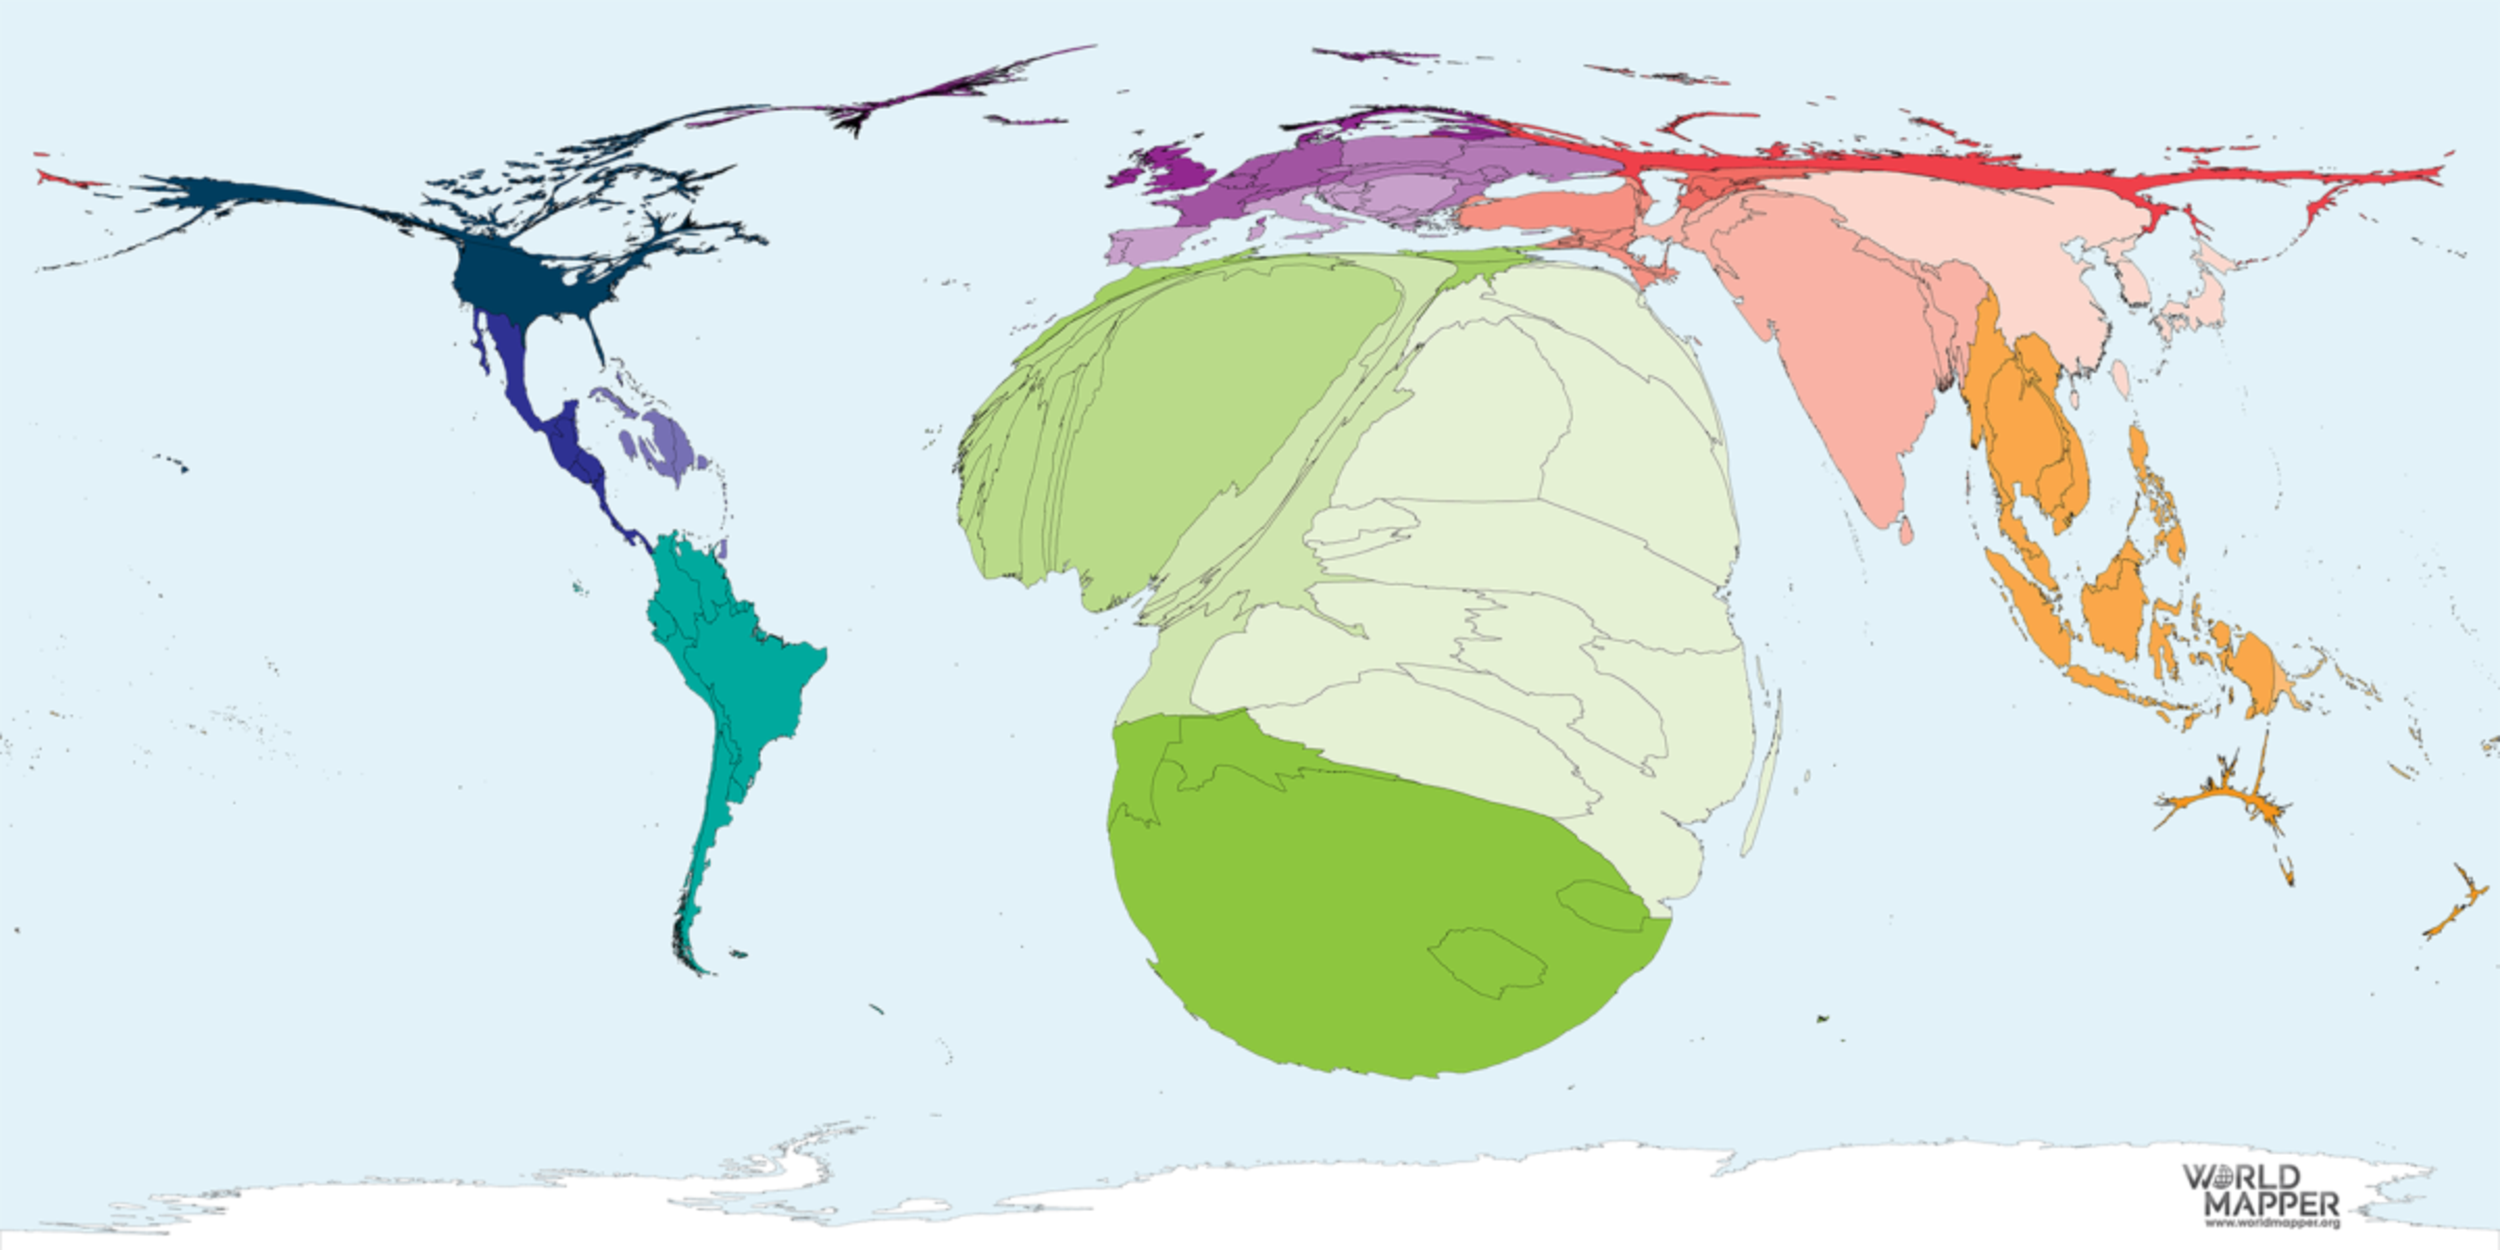
\includegraphics[width=0.65\textwidth]{images/hiv-cartogram}
    
    \begin{itemize}
        \item{Transmission pairs}
        \item{Using genetics to find transmission time}
    \end{itemize}

    \ftnB{Image: GET AN IMAGE CITATION}
    % original was https://www.viewsoftheworld.net/?p=5015
    % new one I found https://worldmapper.org/maps/hiv-prevalence-2013/

\end{frame}

%-------------------------------------------------
\section{What can we expect to see?} % TODO come up with a better title, ugh
%-------------------------------------------------

\begin{frame} \frametitle{\insertsection}
    \begin{center}
        \centering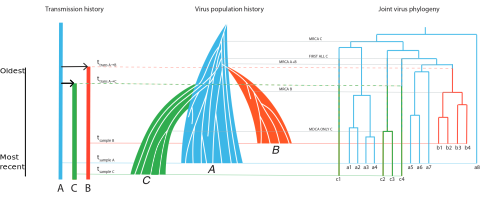
\includegraphics[width=\textwidth]{images/thomas-figure}
        \ftnB{Leitner et al. (2019) Curr. Opin. HIV AIDS}
    \end{center}
\end{frame}

%--------------------------------------------------
\section{Inferring information from a tree}
%--------------------------------------------------

\begin{frame} \frametitle{\insertsection}

    \begin{columns}

        \begin{column}{0.6\textwidth}
            
            \begin{center}
                \centering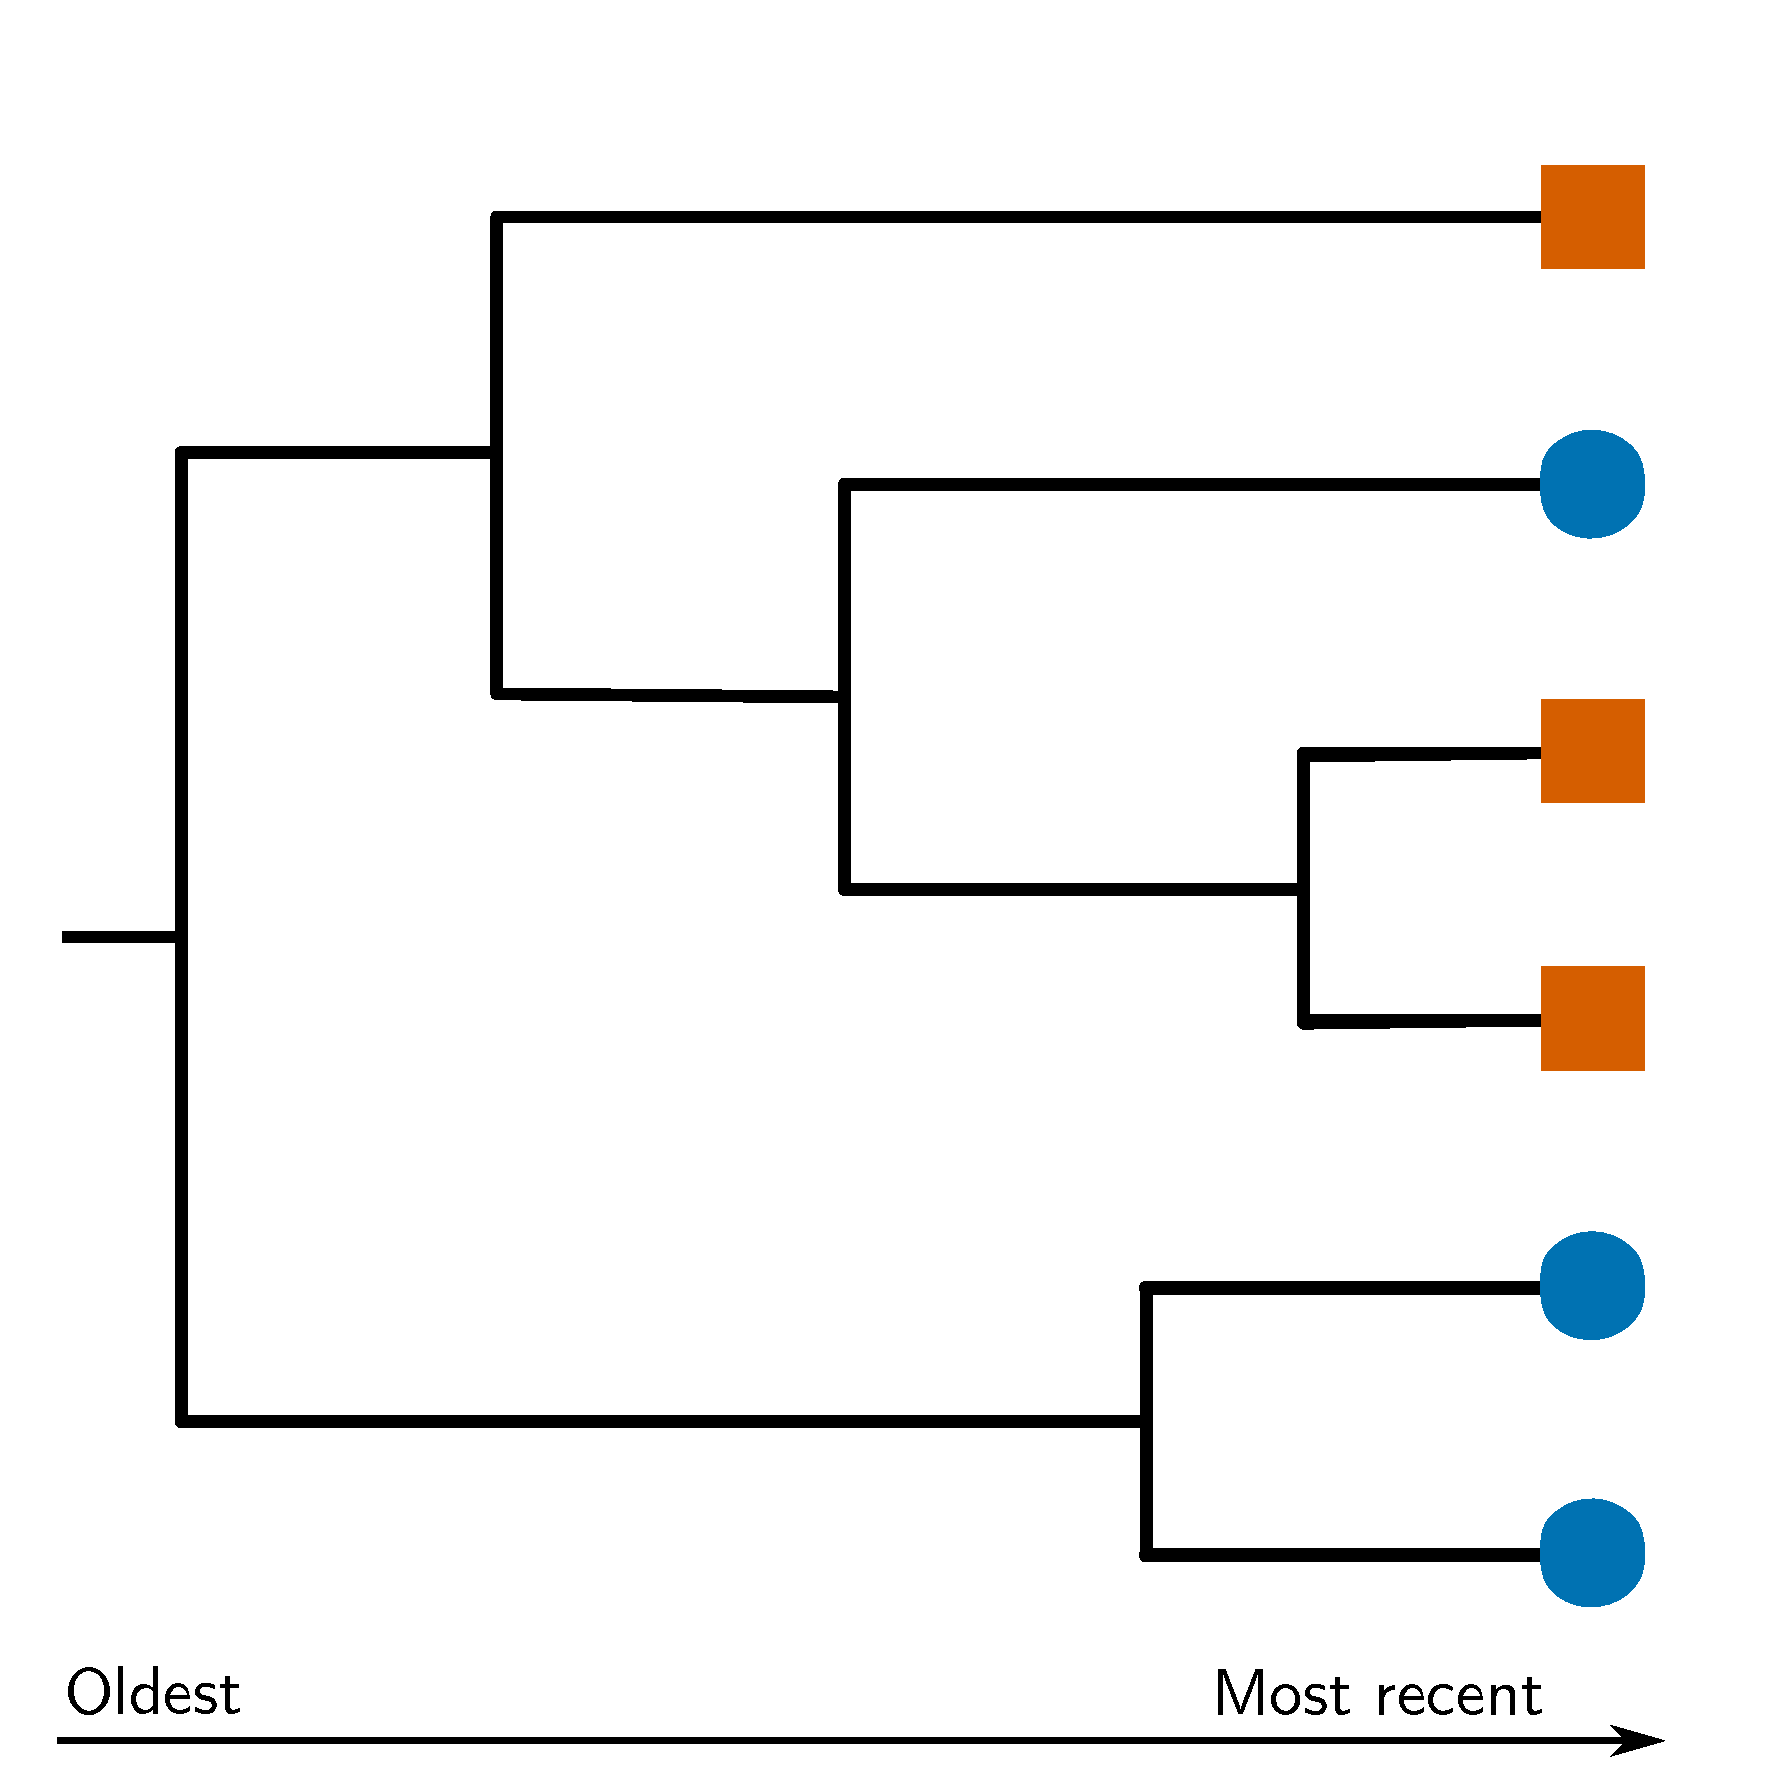
\includegraphics[width=0.8\textwidth]{images/tree-blank}
            \end{center}

        \end{column}

        \begin{column}{0.5\textwidth}

            \begin{itemize}
                \item Tips represent individual viral sequences
                \item Shows the evolutionary distance between individuals
                \item What can we infer about a single transmission time?
            \end{itemize}

        \end{column}

    \end{columns}

\end{frame}

\begin{frame} \frametitle{\insertsection}

    \begin{center}

        \centering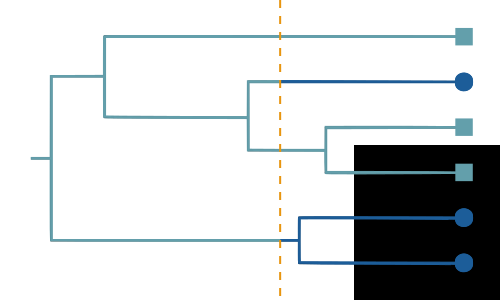
\includegraphics[width=0.8\textwidth]{images/tree-option1}
        
    \end{center}

\end{frame}


\begin{frame} \frametitle{\insertsection}

    \begin{center}

        \centering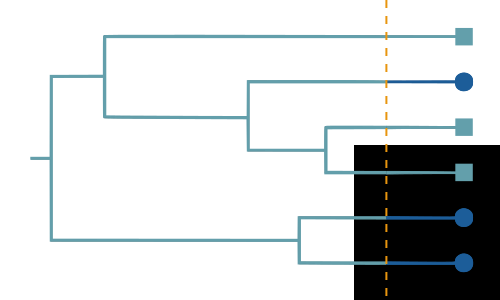
\includegraphics[width=0.8\textwidth]{images/tree-option2}

    \end{center}

\end{frame}


\begin{frame} \frametitle{\insertsection}

    \begin{center}

        \centering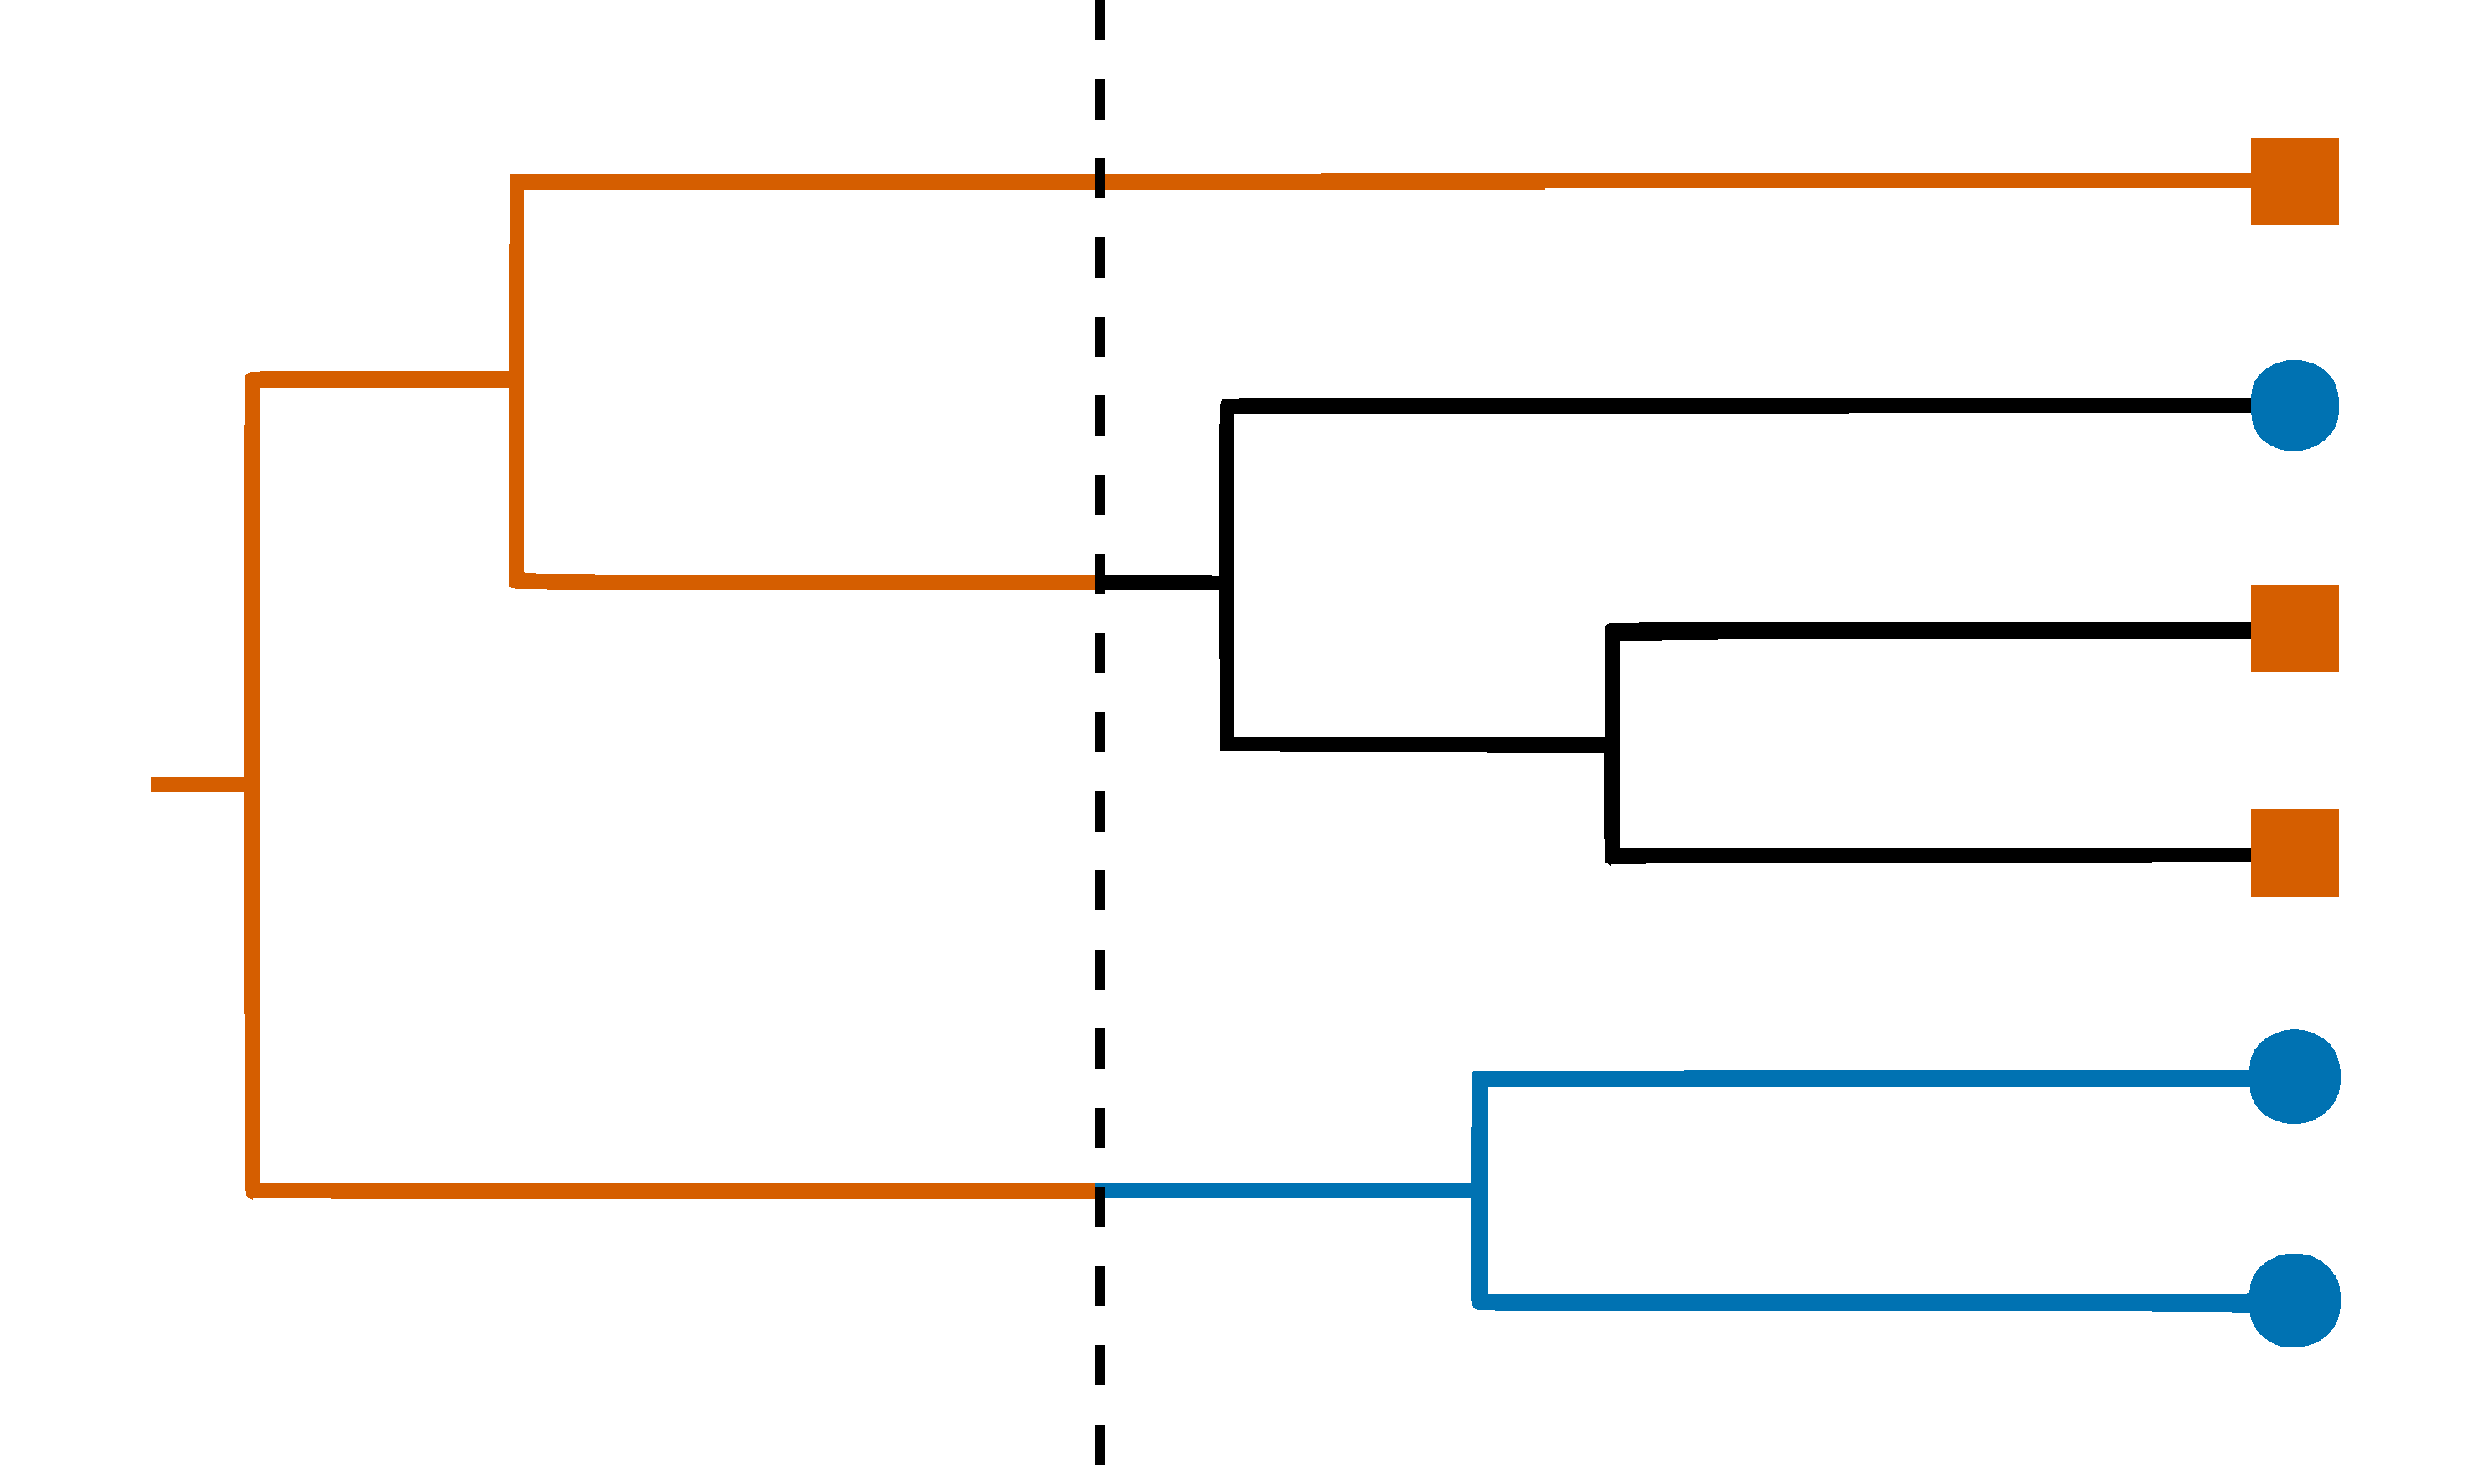
\includegraphics[width=0.8\textwidth]{images/tree-option3}

    \end{center}

\end{frame}


%--------------------------------------------------
\section{Coalescent modeling}
%--------------------------------------------------

\begin{frame} 
    \begin{center}
        \begin{huge}
    
            \textbf{Coalescent modeling:}

            Node times as a function of population size

        \end{huge}
    \end{center}
\end{frame}

%--------------------------------------------------
\section{Relationship between population and samples}
%--------------------------------------------------

\begin{frame} \frametitle{\insertsection}

        \centering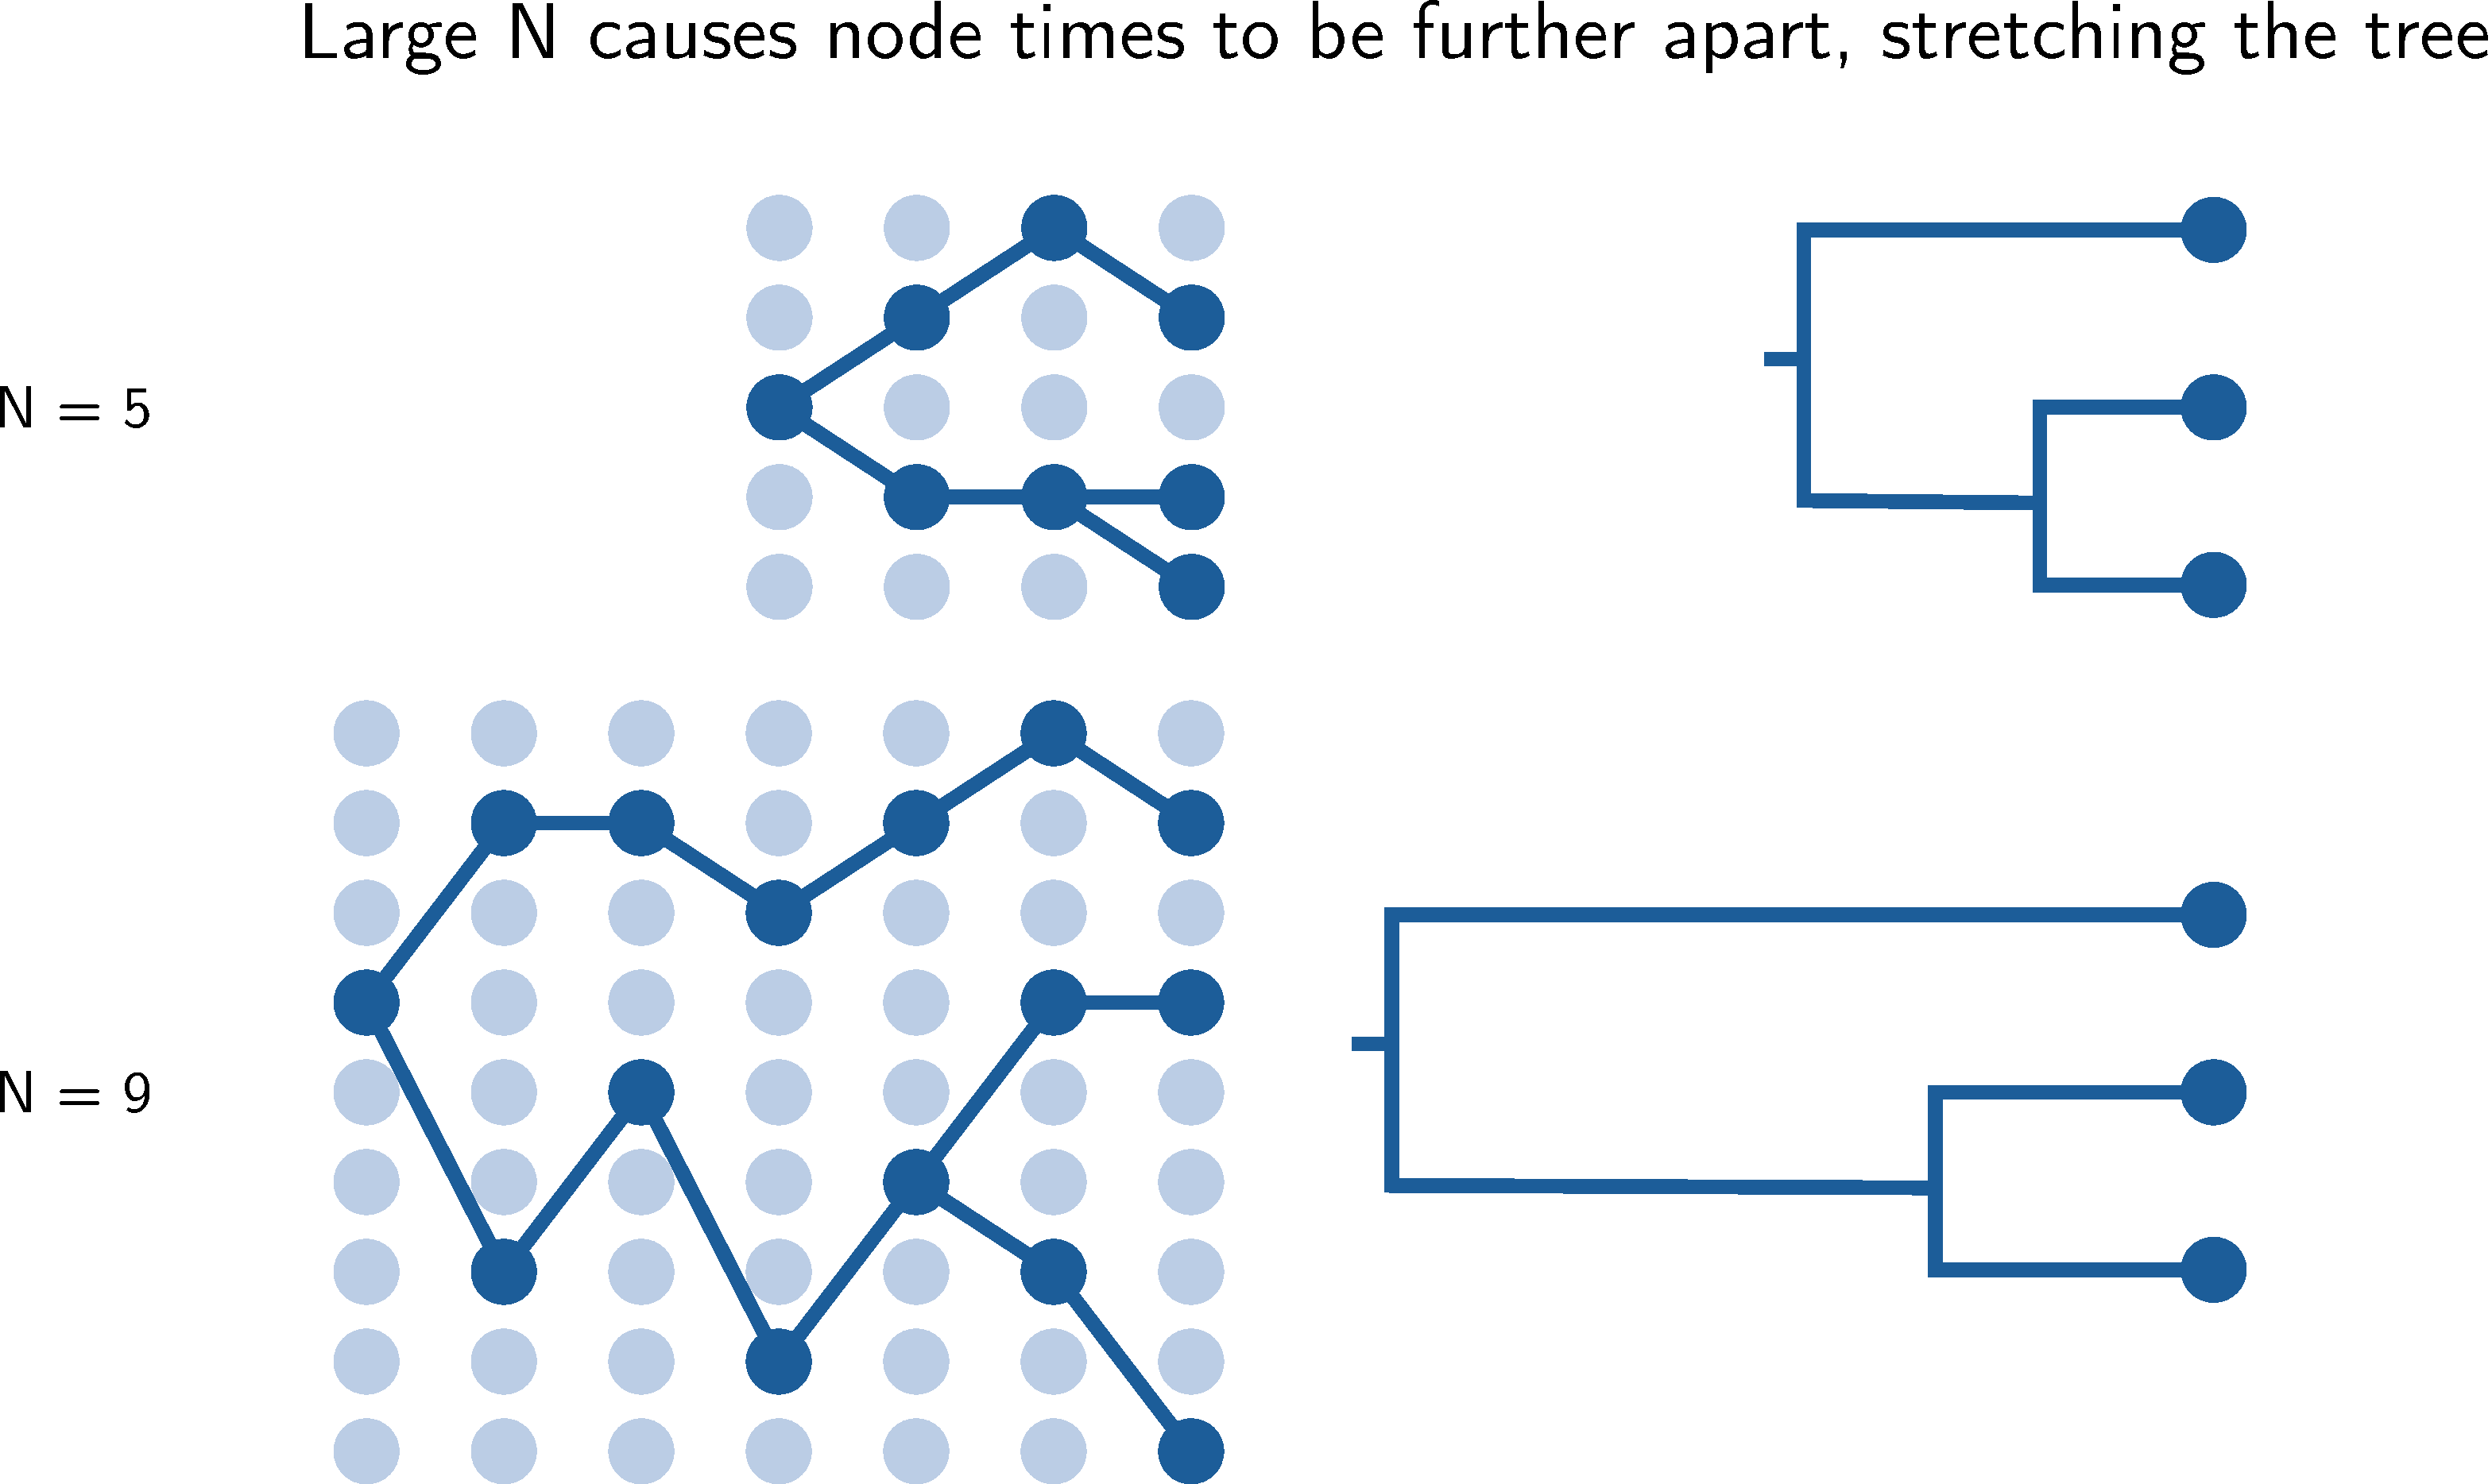
\includegraphics[width=0.8\textwidth]{images/coalescence}

\end{frame}

%--------------------------------------------------
\section{Effect of changing population size}
%--------------------------------------------------

\begin{frame} \frametitle{\insertsection}

    \centering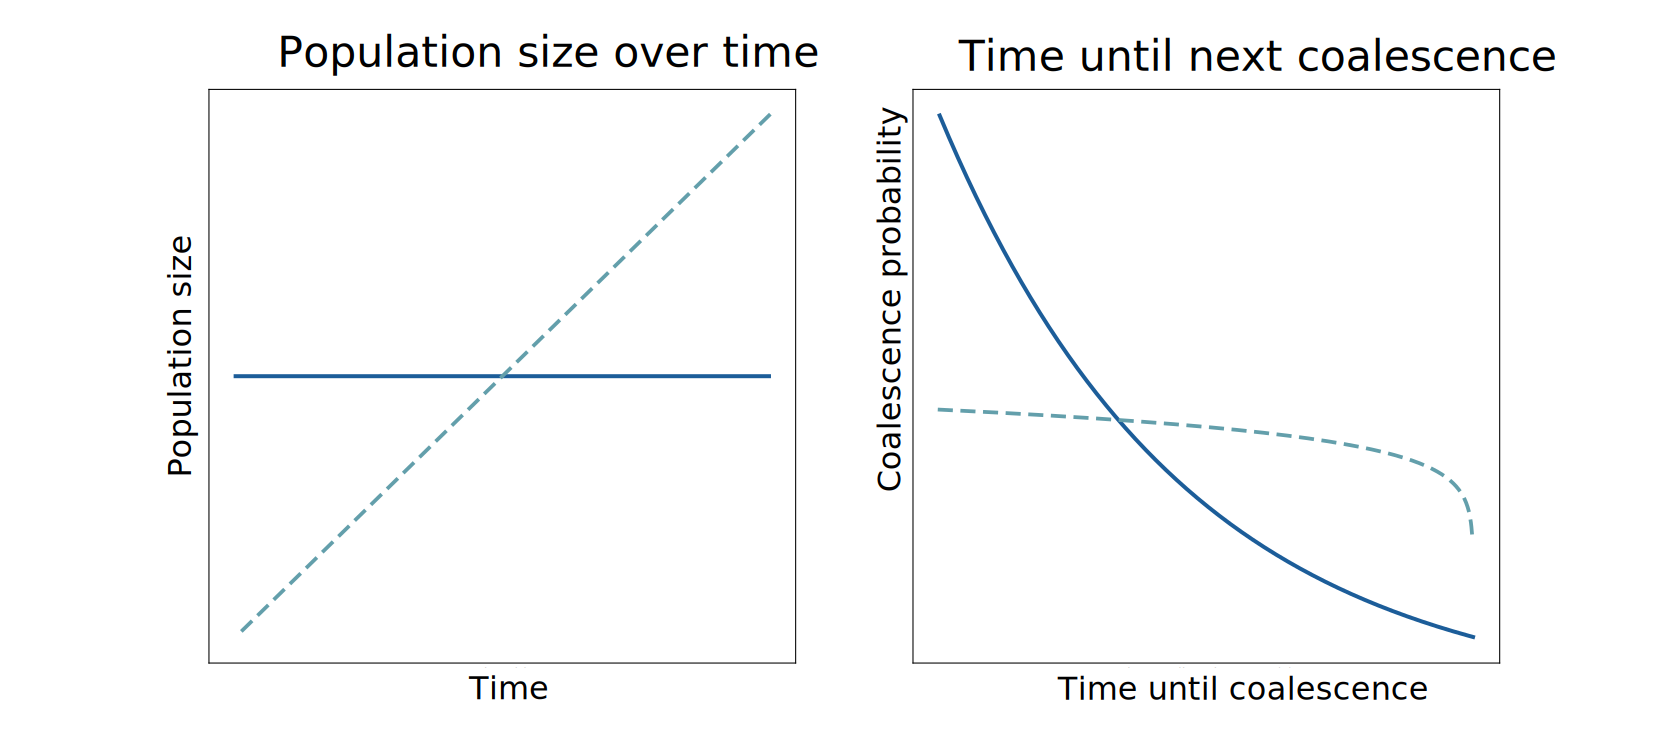
\includegraphics[width=\textwidth]{images/population-comparison}
    % TODO this one is really a mess. Ugh
        
    \ftnB{Romero-Severson et al. (2014) Mol. Biol. Evol.}

\end{frame}

%--------------------------------------------------
\section{Predicting transmission time on a changing population}
%--------------------------------------------------

\begin{frame} \frametitle{\insertsection}

    \centering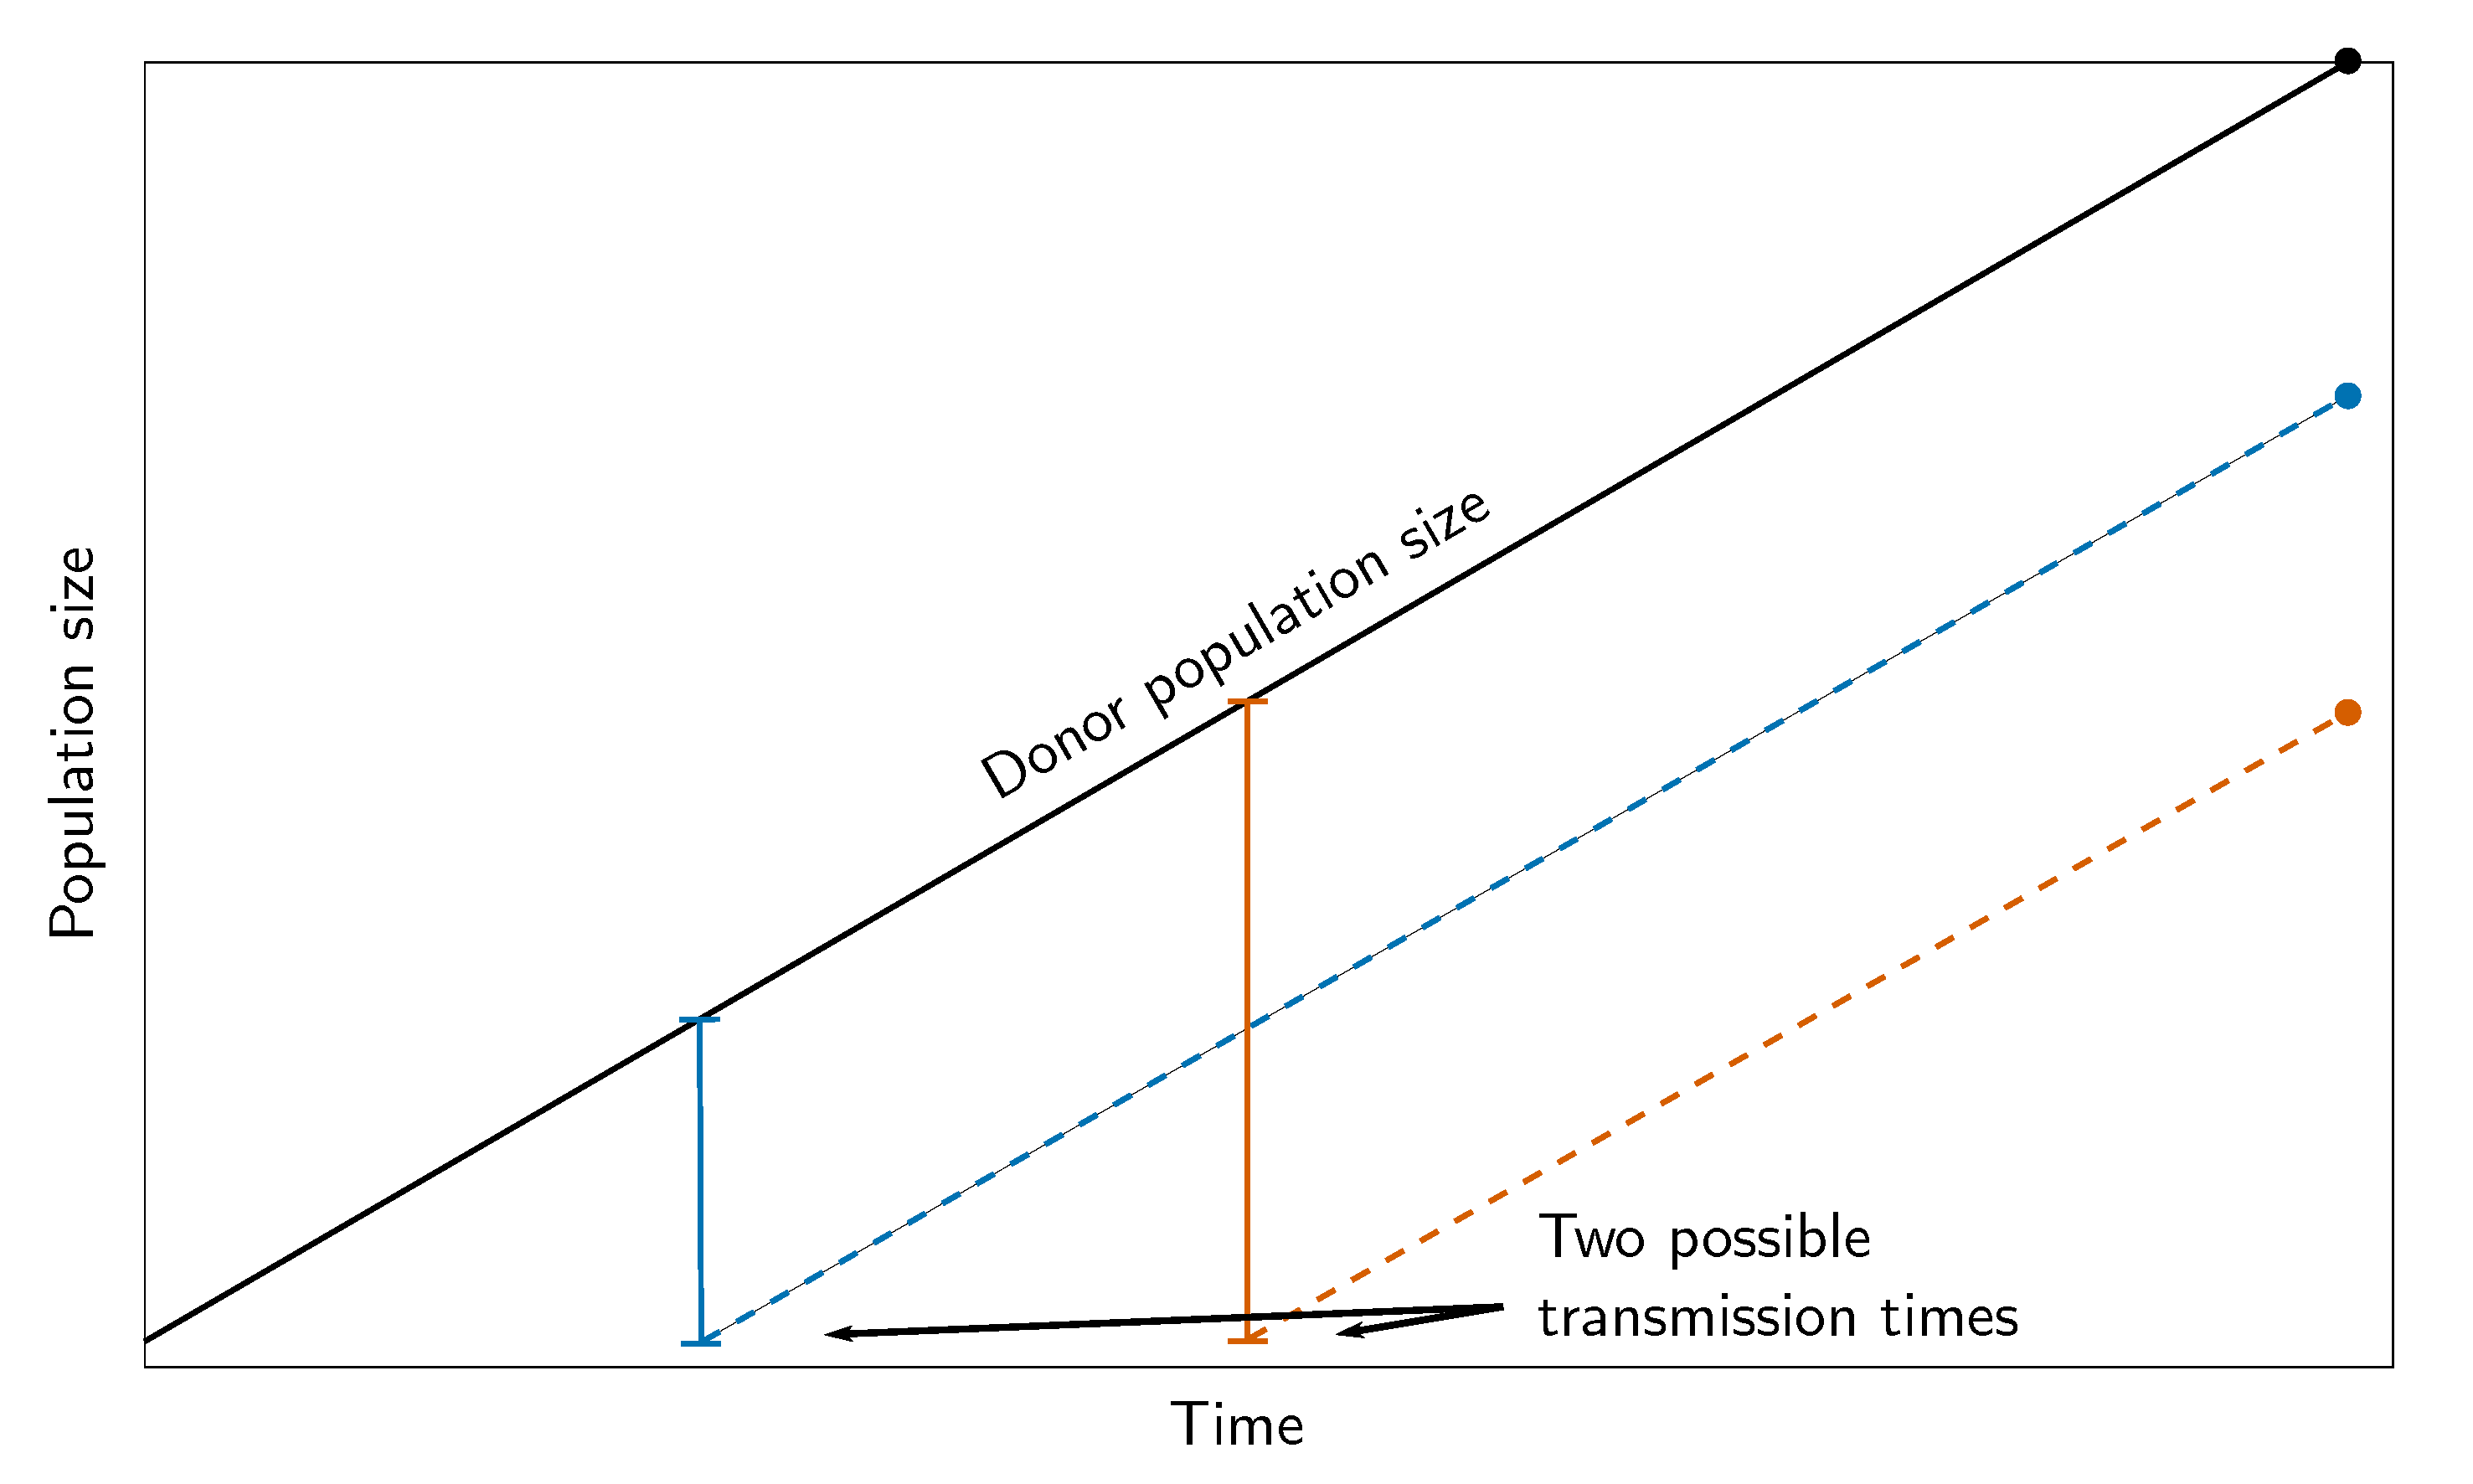
\includegraphics[width=0.8\textwidth]{images/linear-time-location}

\end{frame}

%--------------------------------------------------
\section{Results}
%--------------------------------------------------

\begin{frame} \frametitle{\insertsection}

    What I did\ldots

    In this, I could show what's going on for my 

\end{frame}

%--------------------------------------------------
\section{Next steps}
%--------------------------------------------------

\begin{frame} \frametitle{\insertsection}

    In the coming weeks\ldots

    \begin{itemize}
        \item{Getting linear population to...um, work.}
        \item{What else was I even thinking about lol}
    \end{itemize}

\end{frame}

\begin{frame} \frametitle{\insertsection}

    Next year (and later)\ldots

\end{frame}

\end{document}
